\documentclass[11pt]{article}
\usepackage[letterpaper]{geometry}

\usepackage{tikz-cd}
\usepackage{amsthm}
\usepackage{proof-dashed}
%%% This file can never be completed.
%%% If you need something but cannot find it,
%%% contact the TA Favonia!

%%%%%%%%%%%%%%%%%%%%%%%%%%%%%%%%%%%%%%%%
% Basic packages
%%%%%%%%%%%%%%%%%%%%%%%%%%%%%%%%%%%%%%%%
\usepackage{amsmath,amsthm,amssymb}
\usepackage{fancyhdr}
\usepackage{mathpartir}
\usepackage{xcolor}
\usepackage{hyperref}
\usepackage{xspace}
\usepackage{comment}
\usepackage{url} % for url in bib entries

%%%%%%%%%%%%%%%%%%%%%%%%%%%%%%%%%%%%%%%%
% Acronyms
%%%%%%%%%%%%%%%%%%%%%%%%%%%%%%%%%%%%%%%%
\usepackage[acronym, shortcuts]{glossaries}

\newacronym{HoTT}{HoTT}{homotopy type theory}
\newacronym{IPL}{IPL}{intuitionistic propositional logic}
\newacronym{TT}{TT}{intuitionistic type theory}
\newacronym{LEM}{LEM}{law of the excluded middle}
\newacronym{ITT}{ITT}{intensional type theory}
\newacronym{ETT}{ETT}{extensional type theory}
\newacronym{NNO}{NNO}{natural numbers object}

%%%%%%%%%%%%%%%%%%%%%%%%%%%%%%%%%%%%%%%%
% Fancy page style
%%%%%%%%%%%%%%%%%%%%%%%%%%%%%%%%%%%%%%%%
\pagestyle{fancy}
\newcommand{\metadata}[2]{
  \lhead{}
  \chead{}
  \rhead{\bfseries Homotopy Type Theory}
  \lfoot{#1}
  \cfoot{#2}
  \rfoot{\thepage}
}
\renewcommand{\headrulewidth}{0.4pt}
\renewcommand{\footrulewidth}{0.4pt}


\newcommand*{\vocab}[1]{\emph{#1}}
\newcommand*{\latin}[1]{\textit{#1}}

%%%%%%%%%%%%%%%%%%%%%%%%%%%%%%%%%%%%%%%%
% Customize list enviroonments
%%%%%%%%%%%%%%%%%%%%%%%%%%%%%%%%%%%%%%%%
% package to customize three basic list environments: enumerate, itemize and description.
\usepackage{enumitem}
\setitemize{noitemsep, topsep=0pt, leftmargin=*}
\setenumerate{noitemsep, topsep=0pt, leftmargin=*}
\setdescription{noitemsep, topsep=0pt, leftmargin=*}

%%%%%%%%%%%%%%%%%%%%%%%%%%%%%%%%%%%%%%%%
% Some really basic macros.
% (Lots of them were stolen from HoTT/Book.)
% See macros.tex in HoTT/book.
%%%%%%%%%%%%%%%%%%%%%%%%%%%%%%%%%%%%%%%%
\newcommand*{\ctx}{\Gamma}
\newcommand{\entails}{\vdash}


\newcommand*{\judgmentfont}[1]{{\normalfont\sffamily #1}}
\newcommand*{\postfixjudgment}[1]{%
  \relax\ifnum\lastnodetype>0\mskip\medmuskip\fi
  \text{\judgmentfont{#1}}%
}
\newcommand*{\prop}{\postfixjudgment{prop}}
\newcommand*{\true}{\postfixjudgment{true}}
\newcommand*{\type}{\postfixjudgment{type}}
\newcommand*{\context}{\postfixjudgment{ctx}}


\newcommand*{\truth}{\top}
\newcommand*{\conj}{\wedge}
\newcommand*{\disj}{\vee}
\newcommand*{\falsehood}{\bot}
\newcommand*{\imp}{\supset}


%%% Judgmental equality
\newcommand{\jdeq}{\equiv}
%%% Definition
\newcommand{\defeq}{\vcentcolon\equiv}
%%% Binary sums
\newcommand{\inlsym}{{\mathsf{inl}}}
\newcommand{\inrsym}{{\mathsf{inr}}}
\newcommand{\inl}{\ensuremath\inlsym\xspace}
\newcommand{\inr}{\ensuremath\inrsym\xspace}
%%% Booleans
\newcommand{\ttsym}{{\mathsf{tt}}}
\newcommand{\ffsym}{{\mathsf{ff}}}
%\newcommand{\ttrue}{\ensuremath\ttsym\xspace}
%\newcommand{\ffalse}{\ensuremath\ffsym\xspace}
%%% Pairs
\newcommand{\pair}{\ensuremath{\mathsf{pair}}\xspace}
\newcommand{\tuple}[2]{(#1,#2)}
\newcommand{\proj}[1]{\ensuremath{\mathsf{pr}_{#1}}\xspace}
\newcommand{\fst}{\ensuremath{\proj1}\xspace}
\newcommand{\snd}{\ensuremath{\proj2}\xspace}
%%% Path concatenation
\newcommand{\concat}{%
  \mathchoice{\mathbin{\raisebox{0.5ex}{$\displaystyle\centerdot$}}}%
  {\mathbin{\raisebox{0.5ex}{$\centerdot$}}}%
  {\mathbin{\raisebox{0.25ex}{$\scriptstyle\,\centerdot\,$}}}%
  {\mathbin{\raisebox{0.1ex}{$\scriptscriptstyle\,\centerdot\,$}}}
}
%%% Transport (covariant)
\newcommand{\trans}[2]{\ensuremath{{#1}_{*}\mathopen{}\left({#2}\right)\mathclose{}}\xspace}
% Natural numbers objects
\newcommand{\Nat}{\mathsf{Nat}}
\newcommand{\rec}{\ensuremath{\mathsf{rec}}\xspace}
% Sequence
\newcommand{\Seq}{\ensuremath{\mathsf{Seq}}\xspace}
% Identity type
\newcommand{\Id}[1]{\ensuremath{\mathsf{Id}_{#1}}\xspace}
% Reflection
\newcommand{\refl}[1]{\ensuremath{\mathsf{refl}_{#1}}\xspace}

% fst,snd,case,id
\renewcommand*{\fst}{\textsf{fst}}
\renewcommand*{\snd}{\textsf{snd}}
\DeclareMathOperator{\case}{\textsf{case}}
\DeclareMathOperator{\caseif}{\textsf{if}}
\DeclareMathOperator{\casesplit}{\textsf{split}}
\DeclareMathOperator{\ttrue}{\textsf{tt}\xspace}
\DeclareMathOperator{\ffalse}{\textsf{ff}\xspace}
\newcommand*{\id}{\textsf{id}}


%\setlength{\inferLineSkip}{4pt}

\metadata{Sojakova and Lee}{2013/11/25}

\newcommand*{\Void}{\mathsf{0}}
\newcommand*{\Unit}{\mathsf{1}}
\newcommand*{\Bool}{\mathsf{2}}

\newcommand*{\Interval}{I}
\newcommand*{\Izero}{0_I}
\newcommand*{\Ione}{1_I}
\newcommand*{\Iseg}{\mathsf{seg}}

\newcommand*{\ap}{\mathsf{ap}}
\newcommand*{\dap}{\mathsf{dap}}

\newcommand*{\funext}{\mathsf{funext}}
\newcommand*{\isSet}{\mathsf{isSet}}

\newcommand*{\z}{0}
\newcommand*{\s}{\mathsf{succ}}

\newcommand*{\dummy}{\_}
\newcommand*{\triv}{\langle \rangle}

\newcommand*{\comp}{\circ}

\newcommand*{\W}{\mathsf{W}}
\newcommand*{\wrec}{\mathsf{wrec}}
\newcommand*{\wind}{\mathsf{wind}}

\newcommand{\U}{\mathcal{U}}
\newcommand{\one}{\mathbf{1}}
\newcommand{\two}{\mathbf{2}}
\newcommand{\Sphere}[1]{\mathbb{S}^#1}
\newcommand{\susp}{\ensuremath{\mathsf{susp}}\xspace}
\newcommand{\mer}{\ensuremath{\mathsf{mer}}\xspace}


\newtheorem{lemma}{Lemma}
\newtheorem*{exercise}{Exercise}

\title{15-819 Homotopy Type Theory\\Lecture Notes}
\author{Kristina Sojakova and Joseph Lee}
\date{November 25, 2013}

\begin{document}

\maketitle

\section{Higher Inductive Types}
Recall last week we discussed (lower) inductive types and their definitions. This week,
we move on to discussing higher inductive types. Intuitively, a higher inductive type (i.e. HIT)
can be seen as a type with inductive definitions along with equational laws.

A higher order type then is a generalization of a free algebraic structure, which would have generators
and equational laws that should be fulfilled. For example, a group given by a set of generators
and relations (e.g. commutativity).

This gives a full higher-dimensional structure which allows us to impose relations in multiple dimensions.
In a proof-relevant environment, this means we get generators and more generators. Or in other words,
because of proof-relevance, equational laws can be seen as generators at a higher dimension.

For example, at the 0-type level, the generators are elements or points. These are called the 0-cells.
Identities between 0-cells would be 1-cells, identities between 1-cells would be 2-cells, and so on.
This allows for a type to be defined over multiple dimensions by the use of n-cells.


\section{The Interval Type $\interval$}
Recall that the interval type $I$ is defined by two points, $0_I$ and $1_I$, along with
an identity \seg. That is, $I$ is defined by the 0-cells
\begin{align*}
\Izero &: I\\
\Ione &: I
\end{align*}
and the 1-cell
\[ \seg : 0_I =_I 1_I \]

The recursor is defined as
\[
\infer[\interval\rec]{
  \ctx\vdash\rec[A](a;b;\beta)(M) : A
}{ \ctx \vdash M : I &
  \ctx\vdash a : A &
  \ctx\vdash b : A &
  \ctx\vdash\beta : a =_A b
}
\]
where the $\beta_0$-rules that should hold (i.e. $\beta$-rules for 0-cells) are
\begin{align*}
\rec[A](a;b;\beta)(0_I)&\equiv a\\
\rec[A](a;b;\beta)(1_I)&\equiv b
\end{align*}
and the $\beta_1$-rule is
\[(\ap_{\rec[A](a;b;\beta)}(\seg) =_{a =_A b} \beta) \true\]
That is to say, that the propositional equality above is inhabited.

From here, we can define the induction principle, which is similar to the recursor:
\[
\infer[\interval\ind]{
  \ctx\vdash\ind[z.A](a_0;a_1;p)(M) : A(M)
}{
  \ctx,z:I\vdash A(z):\universe &
        \ctx\vdash M : I &
  \ctx\vdash a_0 : A(0_I) &
  \ctx\vdash a_1 : A(1_I) &
  \ctx\vdash p : a_0 =^{z.A}_\seg a_1
}
\]
Recall that $a_0 =^{z.A}_\seg a_1$ is defined as $\mathsf{tr}[z.A](\seg)(a_0) =_{A(1_I)} a_1$.
This is because $a_0$ and $a_1$ no longer necessarily have the same type, so we need to use "path over"
to express the desired equational law.

The $\beta_0$-rules for induction are
\begin{align*}
\ind[z.A](a_0;a_1;p)(0_I) &\equiv a_0\\
\ind[z.A](a_0;a_1;p)(1_I) &\equiv a_1
\end{align*}
and the $\beta_1$-rule is
\[(\dap_{\ind[z.A](a_0;a_1;p)}(\seg) =_{a_0 =^{z.A}_{\seg} a_1} p) \true\]

There is also a unicity rule, or $\eta$-rule,
that states "if a function behaves like the recursor of $I$, then it
must be the recursor." There is a similar rule for the induction principle of $I$.

\begin{exercise}
Define the $\eta$-rules for $I\rec$ and $I\ind$.
\end{exercise}

\section{The Circle Type $\Sn^1$}
Another example of a higher inductive type is the circle type $\Sn^1$. The $\Sn^1$ type is defined
by the 0-cell (point)
\[ \base : \Sn^1 \]
and the 1-cell (path)
\[ \lloop : \base =_{\Sn^1} \base \]

The recursor is defined as
\[
\infer[\Sn^1\rec]{
  \ctx\vdash\rec[A](a_0;l)(M): A
}{\ctx\vdash M : \Sn^1 &
  \ctx\vdash a_0:A&
  \ctx\vdash l : a_0 =_A a_0
}
\]
with the $\beta_0$-rule is
\[ \rec[A](a_0;l)(\base)\equiv a_0 \]
and the $\beta_1$-rule is
\[ (\ap_{\rec[A](a_0;l)}(\lloop) =_{a_0 =_A a_0} l) \true \]

The induction principle is defined as
\[
\infer[\Sn^1\ind]{
  \ctx\vdash\ind[z.P](b;l)(M) : P(M)
}{
  \ctx,z:\Sn^1\vdash P(z):\universe&
        \ctx\vdash M : \Sn^1 &
  \ctx\vdash b:P(\base)&
  \ctx\vdash l:b =^{z.P}_{\lloop} b
}
\]
with $\beta_0$-rule
\[ \ind[z.P](b;l)(\base) \equiv b \]
and $\beta_1$-rule
\[ (\dap_{\ind[z.P](b;l)}(\lloop) =_{b =^{z.P}_{\lloop} b} l) \true \]
Be careful with the type of $l$, because it is easy to write a type that ``typechecks'' but
is not correct. $l$ should express that taking $b$ around the $\lloop$ path over $P$ returns to $b$.

\begin{exercise}
Define the $\eta$-rules for $\Sn^1\rec$ and $\Sn^1\ind$.
\end{exercise}

\section{Total Space of Loops as a Function from $\Sn^1$}
Recall that we previously characterized the total space of paths,
\[ \int \Id{A} \defeq \sum_{x,y:A}x =_A y\]
as being equivalent to the function type from $I$ to $A$, i.e.
\[ (I\to A) \simeq \int\Id{A} \]
We can similarly characterize the total space of loops
\[ \int\Omega_A\defeq\sum_{x:A}x=_Ax \]
as being equivalent to the function type from $\Sn^1$ to $A$. i.e.
\[ (\Sn^1\to A) \simeq \int\Omega_A\]
\begin{proof}
Define $f : (\Sn^1\to A)\to\int\Omega_A$ as
\[ f = \lambda g.\langle g(\base), \ap_g(\lloop)\rangle \]

\begin{exercise}
Show that $f$ has a quasi-inverse.
\end{exercise}
\end{proof}

\section{Suspensions}\label{}

Another example of a higher inductive type is the \emph{suspension type}, which subsumes the interval and circle types (up to homotopy). For a type $A : \U$, the suspension of $A$, denoted by $\susp(A) : \U$, is the higher inductive type given by two 0-cell constructors 
\begin{align*}
& N : \susp(A) \\
& S: \susp(A)
\end{align*}
which will be referred to as the \emph{north} and \emph{south} poles, respectively, and a family of 1-cell constructors \[\mer : A \to (N =_{\susp(A)} S)\] which can be understood as a collection of \emph{meridians}, i.e., paths from the north to the south pole.

Based on the above data, we can deduce the appropriate recursion schema: given any other type $B : \U$ which "looks like the suspension of $A$", there should be a function, called the recursor, from $\susp(A)$ to $B$, which preserves all the constructors. Expressing this formally, we have the following recursion rule
\begin{mathpar}
\inferrule{\Gamma \vdash B : \U \\ \Gamma \vdash M : \susp(A) \\ \Gamma \vdash b_N : B \\ \Gamma \vdash b_S  : B \\ \\ \\\\ \Gamma, x : A \vdash m(x) : b_N =_B b_S}{\Gamma \vdash \rec[B](b_N;b_S;x.m(x))(M) : B}(\susp(A)\rec)
\end{mathpar}
Furthermore, the recursor behaves according to the following computation rules:
\begin{align*}
\rec[B](b_N;b_S;x.m(x))(N) \equiv b_N : B \\
\rec[B](b_N;b_S;x.m(x))(S) \equiv b_S : B \\
\ap_{\rec[B](b_N;b_S;x.m(x))(-)}(\mer(a)) =_{b_S =_B b_N} m(a)
\end{align*}
The first two computation rules can be considered as $\beta$-rules for the 0-cells and the last one a $\beta$-rule for the 1-cells. Since we do not care about the specific witness term for the propositional equality in the conclusion of the last rule, we simply omit the witness.

We have an analogous induction schema, where instead of simple types $B: \U$ we consider dependent types $E : \susp(A) \to \U$. The induction rule states that in order to construct a dependent function mapping $z : \susp(A)$ to an element of $E(z)$, it suffices to give elements $e_N : E(N)$ and $e_S : E(S)$ such that for each $x : A$, $e_N$ and $e_S$ are associated over the path $\mer(x)$. Formally, this means we have the following induction rule:
\begin{mathpar}
\inferrule{\Gamma, z:\susp(A) \vdash E(z) : \U \\ \Gamma \vdash M : \susp(A) \\ \Gamma \vdash e_N : E(N) \\ \Gamma \vdash e_S  : E(S) \\ \\ \\\\ \Gamma \vdash,x : A \vdash m(x) : e_N =^{z.E(z)}_{\mer(x)} e_S}{\Gamma \vdash \ind[z.E(z)](e_N;e_S;x.m(x))(M) : E(M)} 
\end{mathpar}
Likewise, we have the following computation rules:
\begin{align*}
\ind[z.E(z)](e_N;e_S;x.m(x))(N) \equiv e_N : E(N) \\
\ind[z.E(z)](e_N;e_S;x.m(x))(S) \equiv e_S : E(S) \\
\dap_{\ind[z.E(z)](e_N;e_S;x.m(x))(-)}(\mer(a)) =_{e_N =^{z.E(z)}_{\mer(x)} e_S} m(a)
\end{align*}
where the conclusion of the last rule refers to the application of a dependent function to a path, denoted by $\dap$. We can state and prove a useful uniqueness principle, also known as the $\eta$-rule, asserting that "if a function behaves like the inductor, then it must be the inductor". We leave the exact statement of this principle and its proof as an exercise.

Why are we interested in suspensions in the first place? Interestingly, many familiar (and also not so familiar) inductive types can be characterized as suspensions. For example:
\begin{exercise}
Show that the type $\susp(\zero)$ is equivalent to the type $\two$.
\end{exercise}

\begin{exercise}
Show that the type $\susp(\one)$ is equivalent to the interval type $I$.
\end{exercise}

What is $\susp(2)$? Since the type $\two$ contains only two elements (up to homotopy), we can picture $\susp(2)$ as a type generated by the two points $N$ and $S$ with two distinct paths between them, called \emph{w} and \emph{e}:
\[
  \begin{tikzcd}
     N \arrow[bend right = 65]{d}[swap]{w}\arrow[bend left = 65]{d}{e} \\ 
     S  
  \end{tikzcd}
\]
This of course looks very much like a circle - and indeed it is!

\begin{exercise}
Show that the type $\susp(\two)$ is equivalent to the circle type $\Sphere{1}$.
\end{exercise}

Now we can ask the question, what is $\susp(\susp(2))$? The type $\susp(\susp(2))$ will of course have to contain the two points $N$ and $S$. A function from $\susp(2)$ to the path space $N = S$ can then be thought of as a quadruple $(w, e, \gamma, \delta)$, where \emph{w,e} are two distinct paths from $N$ to $S$ and $\gamma,\delta$ are two distinct paths from $w$ to $e$. The type $\susp(\susp(2))$ generated by all this data can then be visualized as in Fig.~1:
\begin{figure}[t]
\centering
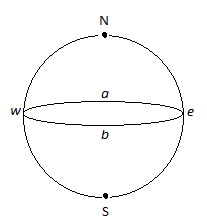
\includegraphics[scale=0.5]{sphere.png}
\caption{$\Sn^{2}$}
\end{figure}

This looks very much like a sphere - hence we can simply make the definition $\Sphere{2} \defeq \susp(\Sphere{1})$. We can iterate this and set $\Sphere{{n+1}} \defeq \susp(\Sphere{n})$.
\end{document}